\section{Introduction}
	\paragraph{}
Characterising the internet through measurements has become very important to both end users and network
managers. Most end users want to know what is causing their network based applications to slow down or take too long to respond. On the other hand network managers want to troubleshoot and detect faulty nodes in a network. The rise of cyber attacks and abuse of networks also makes it of paramount importance for network managers to continuously keep track of what is happening in their network.
\paragraph{}
The goal of this is to present the design and creation of a visualiser for a quality of service monitoring platform for community networks. Such a visualiser is important in that it can help in monitoring network activity and identifying anomalous behaviour.
\paragraph{}
The platform is built as case study for the iNethi community network at ocean view. There are two main types of target users for this platform. The first ones are non-technical end-users of the network. These are people who live in the community and use the network for different purposes. The second group are technical(advanced) end-users with a working knowledge of networking protocols. These would include networking researchers from tertiary institutions and network managers.
\paragraph{}
For non-technical users, the goal of the platform is to enable them to get various statistics calculated based on their past network usage. These statistics will also include websites or services which consumes most of their data and the services they visit the most.
\paragraph{}
On the other hand, the goal for technical users, is to allow them run different measurements on the network with intention to monitor network activities. The results of the measurements are to be displayed on a rich web based visualiser that employs interactive graphs to present each type of measurement. These measurements are to be run on a number of mobile probes deployed haphazardly on the network. Fig 1 shows how the whole system is to be connected together.

\begin{figure*}
	\centering
	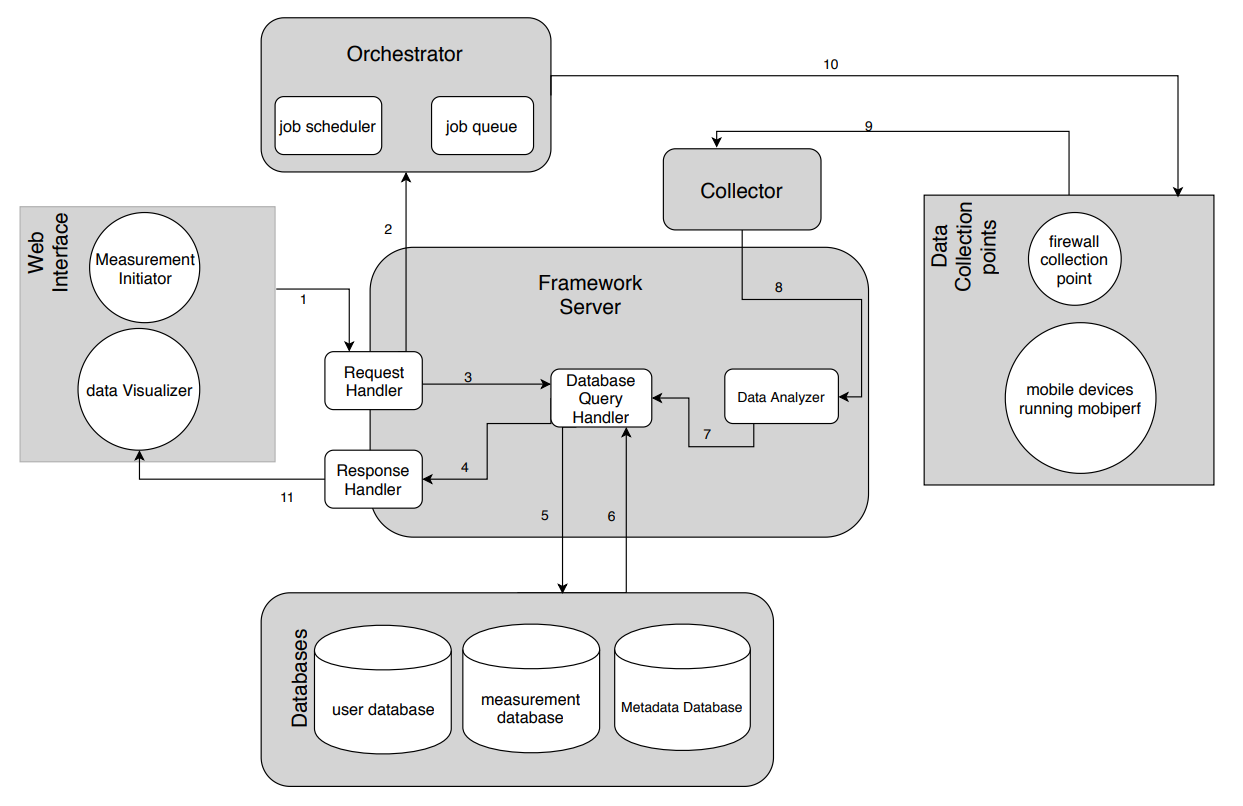
\includegraphics[width=0.7\linewidth]{images/system}
	\caption{Image of the system showing how the visualiser was connected to everything}
	\label{fig:system}
\end{figure*}